%% For double-blind review submission, w/o CCS and ACM Reference (max submission space)
\documentclass[sigplan,10pt,review,anonymous]{acmart}
\settopmatter{printfolios=true,printccs=false,printacmref=false}
%% For double-blind review submission, w/ CCS and ACM Reference
%\documentclass[sigplan,review,anonymous]{acmart}\settopmatter{printfolios=true}
%% For single-blind review submission, w/o CCS and ACM Reference (max submission space)
%\documentclass[sigplan,review]{acmart}\settopmatter{printfolios=true,printccs=false,printacmref=false}
%% For single-blind review submission, w/ CCS and ACM Reference
%\documentclass[sigplan,review]{acmart}\settopmatter{printfolios=true}
%% For final camera-ready submission, w/ required CCS and ACM Reference
%\documentclass[sigplan]{acmart}\settopmatter{}

\usepackage{enumitem}
\usepackage{booktabs}
\usepackage{amssymb}
\usepackage{soul}
\usepackage{xspace}
\usepackage{color}
\usepackage{xcolor}
\usepackage{upquote}
\usepackage{listings}
\usepackage{amsmath}
\usepackage{cleveref}
\usepackage{wrapfig}

\captionsetup[figure]{font=footnotesize,name={Fig.},labelfont={bf, footnotesize}}
\captionsetup[table]{font=footnotesize,name={Tab.},labelfont={bf, footnotesize}, skip=2pt, aboveskip=2pt}
\captionsetup{font=footnotesize,labelfont={bf, footnotesize}, belowskip=2pt}

\newcommand{\eg}{{\em e.g.}, }
\newcommand{\ie}{{\em i.e.}, }
\newcommand{\etc}{{\em etc.}\xspace}
\newcommand{\vs}{{\em vs.} }
\newcommand{\cmpn}{compartmentalization} 
\newcommand{\heading}[1]{\vspace{4pt}\noindent\textbf{#1}\enspace}
\newcommand{\ttt}[1]{\texttt{\small #1}}
\newcommand{\ttiny}[1]{\texttt{\scriptsize #1}}
\newcommand{\spol}[1]{\scriptsize{\sc#1}}
\newcommand{\pol}[1]{\texttt{\small {\color{purple}#1}}}
\newcommand{\rf}[1]{\ref{#1}}
\newcommand{\wka}{\ttt{a\textsubscript{1}}}
\newcommand{\wkq}{\ttt{q\textsubscript{1-4}}}

% For comments
\newcommand{\eat}[1]{}
\newcommand{\TODO}[1]{\hl{\textbf{TODO:} #1}\xspace}
\newcommand{\todo}[1]{\hl{#1}\xspace}
\newcommand{\nv}[1]{[{\color{cyan}#1 --- Nikos}]}
\newcommand{\kk}[1]{[{\color{magenta}#1 --- KK}]}
\newcommand{\review}[1]{{\color{red}#1}}

\definecolor{editorGray}{rgb}{0.95, 0.95, 0.95}
\definecolor{editorOcher}{rgb}{1, 0.5, 0} % #FF7F00 -> rgb(239, 169, 0)
\definecolor{editorGreen}{rgb}{0, 0.5, 0} % #007C00 -> rgb(0, 124, 0)

\definecolor{cdb}{rgb}{0.37, 0.62, 0.63} % cadet blue

\lstdefinelanguage{sh}{
  morekeywords={for, in, do, done, \|},
  keywordstyle=\color{purple}\ttfamily,
  % ndkeywords={curl, grep, wget, awk, xargs, find, nc, mdc, gunzip, cut, sort, head, join},
  ndkeywordstyle=\color{black}\ttfamily\bfseries,
  identifierstyle=\color{black},
  sensitive=false,
  comment=[l]{\#},
  commentstyle=\color{lightgray},
% morecomment=[s]{/\\*\\*, \\*/},
  stringstyle=\color{darkgray}\ttfamily,
  morestring=[b]',
  morestring=[b]",
% numbersep=1pt,
% numberstyle=\footnotesize\bf\color{gray},   % the style that is used for the line-numbers
  abovecaptionskip=0pt,
  aboveskip=0pt,
  belowcaptionskip=0pt,
  belowskip=0pt,
  frame=none                     % adds a frame around the code
% moredelim=[s][\color{gray}]{c:}{>},
% moredelim=[s][\color{orange}]{/*}{/}
}

\lstset{ %
  backgroundcolor=\color{white},   % choose the background color; you must add \usepackage{color} or \usepackage{xcolor}
  basicstyle=\small\ttfamily,  % the size of the fonts that are used for the code
  upquote=true,
  captionpos=b,                    % sets the caption-position to bottom
% frame=B,                    % adds a frame around the code
  numbers=left,                    % where to put the line-numbers; possible values are (none, left, right)
  numbersep=2pt,                   % how far the line-numbers are from the code
  numberstyle=\tiny\color{gray},   % the style that is used for the line-numbers
  rulecolor=\color{black},         % if not set, the frame-color may be changed on line-breaks within not-black text (e.g. comments (green here))
  framerule=0pt,
	xleftmargin=0pt,
	xrightmargin=0pt,
	breakindent=0pt,
  aboveskip=0pt,
  framesep=0pt,
  abovecaptionskip=0pt,
  aboveskip=0pt,
  belowcaptionskip=0pt,
  belowskip=0pt,
  frame=none,
  framexbottommargin=0pt,
  resetmargins=true
}



%% Conference information
%% Supplied to authors by publisher for camera-ready submission;
%% use defaults for review submission.
\acmConference[PL'18]{ACM SIGPLAN Conference on Programming Languages}{January 01--03, 2018}{New York, NY, USA}
\acmYear{2018}
\acmISBN{} % \acmISBN{978-x-xxxx-xxxx-x/YY/MM}
\acmDOI{} % \acmDOI{10.1145/nnnnnnn.nnnnnnn}
\startPage{1}

%% Copyright information
%% Supplied to authors (based on authors' rights management selection;
%% see authors.acm.org) by publisher for camera-ready submission;
%% use 'none' for review submission.
\setcopyright{none}
%\setcopyright{acmcopyright}
%\setcopyright{acmlicensed}
%\setcopyright{rightsretained}
%\copyrightyear{2018}           %% If different from \acmYear

%% Bibliography style
\bibliographystyle{ACM-Reference-Format}
%% Citation style
%\citestyle{acmauthoryear}  %% For author/year citations
%\citestyle{acmnumeric}     %% For numeric citations
%\setcitestyle{nosort}      %% With 'acmnumeric', to disable automatic
                            %% sorting of references within a single citation;
                            %% e.g., \cite{Smith99,Carpenter05,Baker12}
                            %% rendered as [14,5,2] rather than [2,5,14].
%\setcitesyle{nocompress}   %% With 'acmnumeric', to disable automatic
                            %% compression of sequential references within a
                            %% single citation;
                            %% e.g., \cite{Baker12,Baker14,Baker16}
                            %% rendered as [2,3,4] rather than [2-4].


%%%%%%%%%%%%%%%%%%%%%%%%%%%%%%%%%%%%%%%%%%%%%%%%%%%%%%%%%%%%%%%%%%%%%%
%% Note: Authors migrating a paper from traditional SIGPLAN
%% proceedings format to PACMPL format must update the
%% '\documentclass' and topmatter commands above; see
%% 'acmart-pacmpl-template.tex'.
%%%%%%%%%%%%%%%%%%%%%%%%%%%%%%%%%%%%%%%%%%%%%%%%%%%%%%%%%%%%%%%%%%%%%%


%% Some recommended packages.
\usepackage{booktabs}   %% For formal tables:
                        %% http://ctan.org/pkg/booktabs
\usepackage{subcaption} %% For complex figures with subfigures/subcaptions
                        %% http://ctan.org/pkg/subcaption


\begin{document}

%% Title information
\title{Distribution-oblivious Programming with Dish}         %% [Short Title] is optional;
% \titlenote{with title note}             %% \titlenote is optional;
%                                         %% can be repeated if necessary;
%                                         %% contents suppressed with 'anonymous'
% \subtitle{Subtitle}                     %% \subtitle is optional
% \subtitlenote{with subtitle note}       %% \subtitlenote is optional;
                                        %% can be repeated if necessary;
                                        %% contents suppressed with 'anonymous'


%% Author information
%% Contents and number of authors suppressed with 'anonymous'.
%% Each author should be introduced by \author, followed by
%% \authornote (optional), \orcid (optional), \affiliation, and
%% \email.
%% An author may have multiple affiliations and/or emails; repeat the
%% appropriate command.
%% Many elements are not rendered, but should be provided for metadata
%% extraction tools.

%% Author with single affiliation.
\author{First1 Last1}
\authornote{with author1 note}          %% \authornote is optional;
                                        %% can be repeated if necessary
\orcid{nnnn-nnnn-nnnn-nnnn}             %% \orcid is optional
\affiliation{
  \position{Position1}
  \department{Department1}              %% \department is recommended
  \institution{Institution1}            %% \institution is required
  \streetaddress{Street1 Address1}
  \city{City1}
  \state{State1}
  \postcode{Post-Code1}
  \country{Country1}                    %% \country is recommended
}
\email{first1.last1@inst1.edu}          %% \email is recommended

%% Author with two affiliations and emails.
\author{First2 Last2}
\authornote{with author2 note}          %% \authornote is optional;
                                        %% can be repeated if necessary
\orcid{nnnn-nnnn-nnnn-nnnn}             %% \orcid is optional
\affiliation{
  \position{Position2a}
  \department{Department2a}             %% \department is recommended
  \institution{Institution2a}           %% \institution is required
  \streetaddress{Street2a Address2a}
  \city{City2a}
  \state{State2a}
  \postcode{Post-Code2a}
  \country{Country2a}                   %% \country is recommended
}
\email{first2.last2@inst2a.com}         %% \email is recommended
\affiliation{
  \position{Position2b}
  \department{Department2b}             %% \department is recommended
  \institution{Institution2b}           %% \institution is required
  \streetaddress{Street3b Address2b}
  \city{City2b}
  \state{State2b}
  \postcode{Post-Code2b}
  \country{Country2b}                   %% \country is recommended
}
\email{first2.last2@inst2b.org}         %% \email is recommended

\newcommand{\cf}[1]{(\emph{Cf}.\S\ref{#1})}
\newcommand{\sx}[1]{(\S\ref{#1})}
\newcommand{\sys}{{\scshape Dish}\xspace}
\newcommand{\unix}{{\scshape Unix}\xspace}

\setlist{noitemsep,leftmargin=10pt,topsep=2pt,parsep=2pt,partopsep=2pt}

%% Abstract
%% Note: \begin{abstract}...\end{abstract} environment must come
%% before \maketitle command
\begin{abstract}
  \nv{placeholder}
  Distributed systems offer notable benefits over centralized ones.
  Reaping these benefits, however, requires programming in a way that makes distribution explicit---\eg via new programming languages, distributed framework interfaces, or distribution annotations.
% 
%   \emph{Distribution-oblivious programming} is a new approach for..?
  This paper presents \sys, a shell variant that automatically and correctly scales out distribution-oblivious shell pipelines. %  with regards to the sequential program.
  % leveraging the insight that such programs already express stream computations, with their stages falling under a few, known distributability classes.
  \sys's insight is that shell pipelines already express stream computations that can automatically distributed.
  To achieve this, \sys
% a series of techniques for automatically 
decomposes primitives into distributability classes,
identifies high-distributability stages,
applies rewriting rules for largest possible subprograms,
and orchestrates the distributed program.
Its runtime component provides orchestration and planning support during the execution of the program.
% 
% Key challenges include 
% surprisingly expressive, 
% maximally distributable subprograms
% 
Experiments for complex pipelines show substantial speedups and the ability to operate on large input datasets, all without any developer input.
\end{abstract}


%% 2012 ACM Computing Classification System (CSS) concepts
%% Generate at 'http://dl.acm.org/ccs/ccs.cfm'.
\begin{CCSXML}
<ccs2012>
<concept>
<concept_id>10011007.10011006.10011008</concept_id>
<concept_desc>Software and its engineering~General programming languages</concept_desc>
<concept_significance>500</concept_significance>
</concept>
<concept>
<concept_id>10003456.10003457.10003521.10003525</concept_id>
<concept_desc>Social and professional topics~History of programming languages</concept_desc>
<concept_significance>300</concept_significance>
</concept>
</ccs2012>
\end{CCSXML}

\ccsdesc[500]{Software and its engineering~General programming languages}
\ccsdesc[300]{Social and professional topics~History of programming languages}
%% End of generated code


%% Keywords
%% comma separated list
% \keywords{keyword1, keyword2, keyword3}  %% \keywords are mandatory in final camera-ready submission


%% \maketitle
%% Note: \maketitle command must come after title commands, author
%% commands, abstract environment, Computing Classification System
%% environment and commands, and keywords command.
\maketitle


\section{Introduction}
\label{intro}

% 1. Shell scripting; pipelines, in particular, are a common abstraction for expressing filters
% They are an easy way to , because they combine a set of assumptions that work well with Unix
% They work great on a single machine, but are difficult to scale out
% Could we fully automate distribution? 
% The key insight is that pipelines already express a domain-specific
% computation that is easily amenable to distribution.
% 

Distributed systems offer significant benefits over their centralized counterparts---for example, they can speed up expensive computations or process data that would not fit into any single machine.
% offer notable benefits over their centralized counterparts:
%   using partitioning and replication, they can process and store data with increased throughput and fault-tolerance.
% Yet, only a minority of developers, employed by the select few companies that deal with massive datasets, have the luxury of engineering software systems with distribution baked in from the start.
% The remaining majority starts by developing and deploying software in a centralized manner---that is, \emph{until} there is a significant change of requirements, such as a load increase.
Despite these benefits, their development remains different from and significantly more difficult than their centralized counterparts.
Whereas anyone can quickly stitch together a Bash script to compute on a single computer, 
  % domain-experts routinely glue scripts together to process and share data. % without the help of a computing expert.
   scaling out to multiple ones requires expert labor around ``point'' solutions with expensive setups, restricted programming interfaces, and exorbitant composition costs~\cite{taurus:14, dios:13, andromeda:15, pywren:17, futuredata:18, nefele:18}.

To understand this sharp contrast, consider calculating term frequencies over a set of input files:

% \begin{lstlisting}[language=sh,float=h,numbers=none]
% cat doc.ms |                   # print input file
% groff -t -e -mandoc -Tascii |  # remove formatting
% col -bx |                      # remove backspaces 
% tr A-Z a-z |                   # convert to lower case
% tr -d '[:punct:]' |            # remove punctuation
% sort |                         # put words in alphabetical order
% unique |                       # remove duplicate words
% comm -13 /usr/share/dict -     # report words not in dictionary 
% \end{lstlisting}

\begin{lstlisting}[language=sh, float=h, numbers=none, escapeinside={($}{$)}]
cat * | tr -cs A-Za-z\n | tr A-Z a-z |    ($$[p_1]$$)
  sort | uniq -c | sort -rn | head 5 > out
\end{lstlisting}

\noindent
Program $p_1$ creates a character stream, breaks it into words, transliterates to lower-case, sorts to group duplicates, summarizes them with a counter, sorts them in descending order, picks the top five results and writes them to a file \ttt{out}.
Combining several features, \unix makes small tasks easy to express;
  for a user with \emph{one} computer and small input, this pipeline takes a few seconds to compose and execute~\cite{bentley1986literate}.
% composition allows the composition of general primitives

% Key insight 
% % The garden-hose philosophy is similar to Haskell 
% This pipeline takes an input file (line 1), removes 
% * do not need to use specialized frameworks for composition---instead, as long as they conform to the shell, individual primitives can be written in any programming language.
% * do not need to rewrite ---

\begin{figure}[t]
\centering
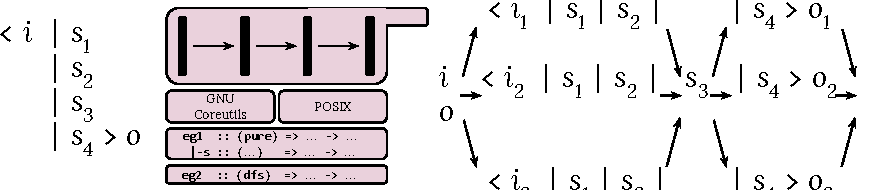
\includegraphics[width=0.49\textwidth]{./figs/dish_schematic.pdf}
\caption{
  \textbf{\sys high-level schematic.}
	\sys XYZ
}
\label{fig:schematic}
\end{figure}


%      dish      ignis, mozart    hadoop, spark, ...      erlang, elixir
%       \/           \   /             \     /                \   /
% auto <-------------------------------------------------------------> manual
%                      [rewrite (not write) cost]

For a user with many computers and larger inputs, however, developing $p_1$'s distributed equivalent requires a significant effort.
% The scope of such rewrites, and therefore the cost of manual effort, can vary considerably.
For simple pipelines that capture in restricted models of computation, this effort amounts to expressing the computation using the primitives provided by a big-data framework~\cite{mapreduce:08, ciel:11, spark:12, naiad:13} or domain-specific language~\cite{alvaro2011consistency, distal:13, meiklejohn2015lasp}---an unjustifiable cost for one-off pipelines that take a few minutes to compose (but are applied to large datasets).
More complex pipelines, such as the ones presented in later sections, require full-fledged distributed programming language~\cite{erlang:96, lopes1997d, acute:05, mace:07, cloudhaskell:11, ScalaLoci:18}. %  or a distributed operating system---\eg Plan9's \ttt{rc} shell.
In these cases, manual rewriting is expensive and can introduce new bugs, cascading changes, or divergence from legacy functionality.
Could the generation and execution of $p_1$'s distributed version be fully and correctly automated?

% Some (parts of) pipelines require only moderate effort, as they are 
% For some pipelines, this effort is merely moderate, as 
%  can be expressed in domain-specific frameworks---for example, Hadoop and Spark provide a few purely functional primitives that 
%   ---still requiring rewriting the program in a different (\eg Scala for Spark).
% 
% This effort is moderate if the program expressed by these pipelines fits into a domain-specific framework.
% At times, such pipelines
% As long as the program fits into the model this is only moderately difficult;
% 
% For many legacy pipelines  
%  has to choose between three options, all of which require significant manual effort.
% The most invasive is to rewrite the entire program in a distributed programming language
% The most popular is to leverage 
% 
% Use a distributed programming language, even higher rewrites
% Or use some form of annotations 
% 
%  this requires rewriting portions of the program in a new language and use operations
% 
% 
% In the simplest case, annotations
% 
% Often, they only focus on a few parts of the system---for example, upgrading to a distributed storage layer.
% More rarely, companies rewrite entire systems (\eg Twitter's Ruby-to-Scala rewrite~\cite{twitter}), a process that is notoriously difficult under schedule constraints and competitive pressures~\cite{rewrite1, rewrite2}.
%  especially since software today makes extensive use of third-party modules~\cite{breakapp:plos:2017}.
% 

% If developers have already expressed their computation as a Unix pipeline, they should not have to manually rewrite the program in other environment---\eg Hadoop, Spark---to exploit distribution.


The key insight behind \sys is that the language of the Unix shell already encodes stream processing, providing most of the information required for distributing a computation.
\sys builds on this insight with a careful study of the scalability properties of shell primitives and its commands, paired with a novel rewriting scheme that identifies maximal pipeline sub-expressions that are candidates for scale-out.
We term the result \emph{distribution-oblivious programming}---a series of techniques that fully automates program distribution while provably maintaining correct (non-distributed) semantics.

Key benefits include the ability to scale legacy computations onto
\sys converts legacy shell pipelines into their distributed equivalents fully automatically, offering $100\times$ improvements in performance without a single line of additional code or annotation.
Most importantly, \sys provides an architectural lesson:
  the current design shows that large-scale efforts in the distributed- and operating-system literature to provide a \unix-like distributed equivalent could have been simplified by a thin (but sophisticated) rewriting shim like the one \sys provides.

% % Make Unix benefits explicit?
% Indeed, the primary reason behind $p_1$'s succinctness is that the pipeline is a domain-specific language for describing operations over streams.
% Key elements of \unix are the ability to compose programs written in different languages, the abstraction of a file system as a set of resident streams, a small but extensible library of commands, and the ability to resolve names within a global context.
% Under the hood, the \unix kernel buffers results, synchronizes processing stages, and generally orchestrates the computation.

% Primitives 
% \sys enables \emph{distribution-oblivious programming}: 
%   multi-order of magnitude speedups with correctness guarantees and without any developer effort.
% 
% The a series of transformations that 
% Second, we are using describing composition . For this, we are restricting the study to a subset of the POSIX shell--
% 
% Local operations and identifiers have to be carefully translated to distributed ones, a translation that depends on the types of the operations and associated identifiers.
% 
% The semantics is enough to capture powerful features such as stream branching and feedback constructs found in practice and in the system's evaluation.

The paper is structured as follows.
We first start with a background section outlining pipeline concepts~\sx{bg}.
Sections \ref{classes}--\ref{recipes} highlight our key contributions:\footnote{
  This is not precise, we'll need to wait until it matures a bit.
}
\begin{itemize}

  \item
  \S\ref{classes} overviews \sys and introduces several scalability and distributability classes.

  \item
  \S\ref{rewrite} presents a set of rewriting transformations for identifying maximal pipeline sub-expressions, candidates for scale-out.

  \item
  \S\ref{other} details other concerns, such as distributed state management and extensibility.
\end{itemize}

\noindent
\sys's evaluation~\sx{eval} uses a combination of one-liner micro-benchmarks that highlight certain features and three multi-line macro-benchmarks---a web crawling and indexing engine, a production genomics pipeline, and a large-scale weather analysis.
We close with a discussion of related prior work~\sx{related} and possible future directions~\sx{discussion}.

% \begin{figure*}[t]
% \centering
% 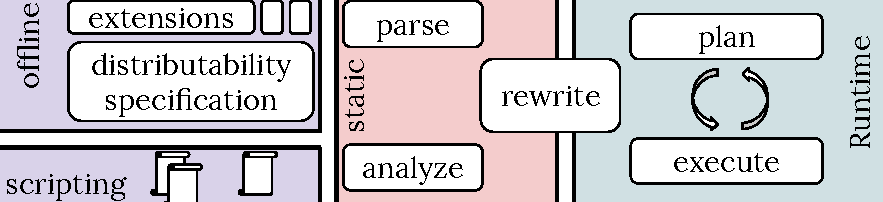
\includegraphics[width=0.49\textwidth]{./figs/dish_overview.pdf}
% \caption{
%   \textbf{Applying \sys to $p_1$.}
% }
% \label{fig:example}
% \end{figure*}
% 

\section{Background}
\label{bg}

This section breaks down $p_1$ to presents important background on and challenges
of shell scripting.

\subsection{Unix Composition, Informally}
\label{bg:pipelines}

% A pipeline is a mechanism for program composition that works by chaining together programs (or, \emph{commands}) using pipes.
\unix provides several ways for succinct program composition.
Central among them is the \emph{pipe}, a primitive that passes the output of one program as input to the next.
These programs produce output and consume input concurrently, and possibly at different rates, with the \unix kernel facilitating program scheduling and communication synchronization behind the scenes.
Intermediate programs, termed commands, can also be developed in different programming languages, as long as they conform to a common interface.
\begin{wrapfigure}{r}{0.06\textwidth}
  \vspace{-12pt}
  % \begin{center}
    % \includegraphics[width=0.48\textwidth]{gull}
    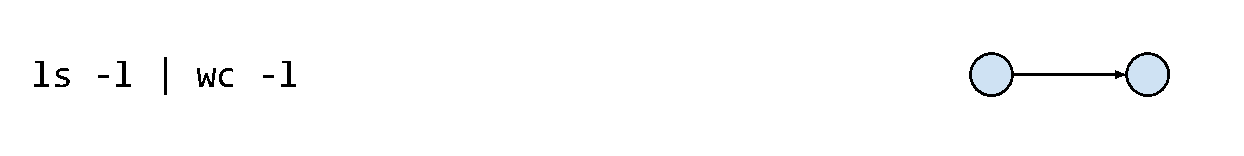
\includegraphics[width=0.06\textwidth]{./figs/dish_ex1.pdf}
  % \end{center}
  \vspace{-30pt}
\end{wrapfigure}
This interface exposes a stream of contiguous character lines.
A few characters are special---for example, the newline (\textsc{NL}) character delineates an element of the stream, and the end-of-file (\textsc{EOF}) character signals the end of a stream.
As part of this interface, each command has access to (any combination of) three \emph{standard} streams---input, output, and error.
% the input stream (stdin), the output stream (stdout), and the generating errors or diagnostics to the standard error stream (stderr)
% generating errors or diagnostics to the standard 
% Leveraging this interface, pipelines chain together commands by their standard streams, such that the output stream of one command (stdout) is passed directly as input (stdin) to the next one.
% TODO: \kk{We have to mention character vs line based parallelism somewhere, and that we choose to see lines as the data quantum}

Commands can be tuned by two mechanisms, namely command-line options and environment variables.
Options control the execution of a program---\eg changing the \ttt{sort}ing order.
The shell does not have any visibility into these options; 
  their parsing and evaluation is left entirely up to each command.
Environment variables carry more general information about the surrounding system---\eg file search paths, system defaults, parsing switches \etc 
They are organized in a map from names to values, both of which are strings, and can be evaluated at any point in the program---including as commands, flags, a shell feature termed parameter \emph{expansion}.

% TODO: Talk about security primitives?
Streams are a key feature of \unix, and go hand-in-hand with the file abstraction:
  files are simply persistent streams that can be manipulated by commands or pipelines.
\begin{wrapfigure}{r}{0.15\textwidth}
  \vspace{-15pt}
  % \begin{center}
    % \includegraphics[width=0.48\textwidth]{gull}
    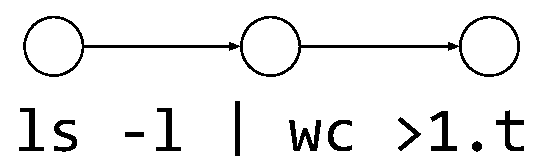
\includegraphics[width=0.15\textwidth]{./figs/dish_ex3.pdf}
  % \end{center}
  \vspace{-25pt}
\end{wrapfigure}
Reading a file or a set of files generates a stream; 
  similarly, streams can be trivially redirected to the file system---by appending with the file identifier.
Files are named, in the sense that they correspond to a global identifier---for example \ttt{cat /x/y} returns the persistent stream associated with the identifier \ttt{/x/y}.
\unix exposes a few different types of files---\eg directories, symbolic links, named pipes (or FIFOs), and special character devices.
As a result, file-system identifiers part of a pipeline may resolve to in-memory structures or pseudo-devices (\eg \ttt{/dev/urandom}).

% At a high level, POSIX defines several file types:
% (-) regular files, storing lines of text or binary data,
% (d) directories, grouping together multiple other files,
% (l) symbolic links, pointing to other files,
% (p) named pipes or FIFOs, communication primitives that can be named and manipulated like files,
% (s) domain sockets or DSes, full-duplex communication primitives that support passing file descriptors, and
% (b or c) special files, interfaces to device drivers or low-level abstractions, presented as ordinary files.

Special files are particularly interesting because they are resolved to OS structures.
One example is the special \ttt{/proc} filesystem (procfs) that presents information about processes and the operating system, offering a feature analogous to programmatic introspection:
  with \ttt{procfs} commands can inspect and alter their directory or the flags passed to them.
% Here are a few examples:
% (i) \ttt{/proc/PID/cmdline} contains the command that originally started the process,
% (ii) \ttt{/proc/modules} contains a list of the kernel modules currently loaded, and
% (iii) \ttt{/proc/PID/cwd} contains a symlink to the current working directory of the process.
Similarly, \unix exposes file-system handles for various ephemeral structures, including standard streams.
This bidirectional relationship between ephemeral streams and persistent names---the fact that streams can be named in the file-system and files can be converted to streams---is a key enabler of the runtime rebinding achieved during our transformations.

A small but powerful set of features is concerned with stream manipulation.
Some of these features are built into the shell;
  for example, given a file identifier, stream redirection operators can direct stdout or stderr to a file.
\begin{wrapfigure}{r}{0.15\textwidth}
  \vspace{-15pt}
  % \begin{center}
    % \includegraphics[width=0.48\textwidth]{gull}
    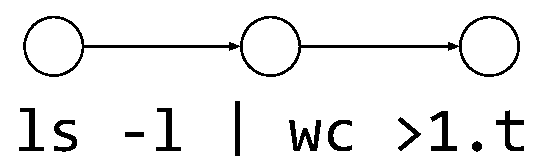
\includegraphics[width=0.15\textwidth]{./figs/dish_ex3.pdf}
  % \end{center}
  \vspace{-25pt}
\end{wrapfigure}
As described before, the file can be a FIFO dubbing as input to another command.
More interestingly, some commands allow splitting (resp. merging) a single stream (resp. many streams) into multiple streams (resp. a single stream);
  stream merging can be achieved by appending one stream after the end of another or by fusing (zipping) streams column-wise into a single (fat) stream.
% TODO: talk about \ttt{xargs}?

% Explicit Redirection, Implicit splitting and merging, This can be done through the file-system operators 

The combination of file-system identifiers pointing to ephemeral streams and the stream redirection described above enable surprisingly expressive pipelines. %---for example:
The most interesting feature of these pipelines is the presence of cycles:
  a pipeline segment processes some input, part of which is extracting the next input to process.
One example use case, discussed in the evaluation section~\sx{eval} is a web crawler that feeds extracted URLs from the input stream back to the start of the pipeline.
% These streams are created by the C library (glibc) at the start of program execution,
% and new streams can be created to connect to files, sockets, pipes,

Apart from pipes, the \unix shell provides several other forms of program composition such as sequential (\ttt{;}) and parallel (\ttt{\&}) composition operators.
Command substitution, expressed as \ttt{\$($c$)}, replaces the expression with the results of executing $c$.
Code blocks, expressed as \ttt{\{$c_1; c_2$\}}, can redirect streams for the entire group of $c_1$ and $c_2$;
  this is analogous to an anonymous function, which contains many statements and can possibly be assigned to a variable that can later be invoked with parameters.
Subshells, enclosed in \ttt{($c_1; c_2$)}, are similar to code blocks but spawn a child shell, thus avoiding the pollution of their environment variable context. % but incurring higher overhead.


% \begin{lstlisting}[
%   language=es,
%   mathescape,
%   float=t,
%   belowskip=-5mm,
%   label=core-pl,
%   upquote=true,
%   caption={
%     \textbf{The core language of the POSIX shell.}
%     The language used by ; file identifiers and expansion are not shown.
%   }]
% $p$ ::= $s\in{}String$ | $n\in{}Number$ | $b\in{}Bool$ | $\emptyset$
% $v$ ::= $p$ | ($x$,$\ldots$) => {e} | {$s$:$v$,$\ldots$} | [$v$,$\ldots$]
% $e$ ::= x | $v$ | ($x$ = $e$) $e$ | $e$($e$) | $e$[$e$] = $e$
% \end{lstlisting}

% \begin{lstlisting}[language=sh, float=h, numbers=none, escapeinside={($}{$)}]
%  cat /proc/ >                            (($$p_4$$))
% \end{lstlisting}
% \begin{lstlisting}[language=sh, float=h, numbers=none, escapeinside={($}{$)}]
%  ls -l | wc -l                           (($$p_2$$))
% \end{lstlisting}
% \begin{lstlisting}[language=sh, float=h, numbers=none, escapeinside={($}{$)}]
%  cat * | wc -l > out.txt                 (($$p_3$$))
% \end{lstlisting}
% \begin{lstlisting}[language=sh, float=h, numbers=none, escapeinside={($}{$)}]
%  cat /proc/ >                            (($$p_5$$))
% \end{lstlisting}
% \begin{lstlisting}[language=sh, float=h, numbers=none, escapeinside={($}{$)}]
% { echo 1; echo 2; } > out.txt
% \end{lstlisting}

\begin{figure}[t]
\centering
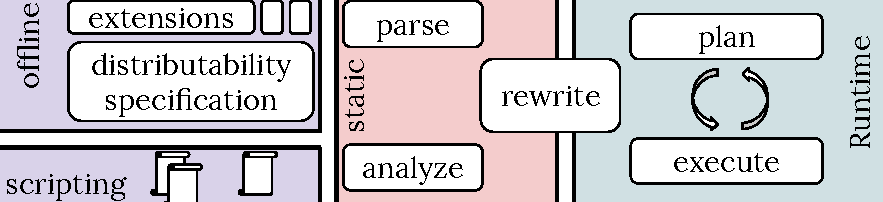
\includegraphics[width=0.49\textwidth]{./figs/dish_overview.pdf}
\caption{
  \textbf{\sys transformation overview.}
	\sys XYZ
}
\label{fig:overview}
\end{figure}


% \heading{Generation}
% Expansion---the key is that expansion and evaluation are handled by the shell at an earlier stage 
% The most powerful---and interesting, for \ttt{dish}---type of expansion is subshell expansion, that allows replacing entire input streams 

\subsection{Overview}

As outlined earlier, the key insight behind \sys is that the shell already describes parallel computations over streams.
Intuitively
 (i) the parallel-composition operator exposes task parallelism,
 (ii) commands such as \ttt{xargs} and \ttt{tee} expose data parallelism,
 (iii) the pipe operator enables both task and data parallelism, and
 (iv)  other composition operators can be viewed as barriers.
To leverage these insights and correctly distribute a pipeline such as $p_1$, \sys must solve several challenges.

Understanding the primitives of the shell is not enough;
  one has to understand the characteristics of commands used to compose larger programs.
This challenge has two parts
One, characterize the commands already in the shell---that is, built-ins .
This study identifies a small set of well-understood distributability classes and is already useful enough to allow the composition of practical pipelines.
The second part is to use these classes to 
Using this language -> extensions
A command developer can only annotate the default behavior;
  if a new flag is added a few years later, and only if that flag alters the command's class, only then a new annotation is needed.

Given a set of , \sys's has to analyze the given pipeline and identify candidate subexpressions for distribution.
\sys addresses this challenge with a dataflow analysis that identifies longest subexpressions.
This analysis is not trivial, as many of the shell's dynamic features have to be taken into consideration---examples include shell expansion, environment variables, file input sizes, \etc

Given a distributed pipeline with runtime instrumentation---two challenges.
First, wrapping 
  just-in-time wrappers for all the, generated by the distributability specification outlined earlier.
The reasoning behind thin wrappers is that they should not interfere with legacy functionality---commands have many flags accumulated over long periods of time.
Second, fill-in planing holes left by the rewriting engine.
This is achieved with \emph{planner activators}, commands yield (passing their arguments) to the scheduler.
From the point of view of the shell, activators are higher-order commands a la \ttt{xargs} and \ttt{time} that take other commands as arguments---a technique that achieves the latest possible binding.

The next few sections , and discuss other challenges such as the synchronization of environment variables, distributed file operation, \etc.


\section{Distributability Classes}

\subsection{Comnands}
\label{bg:cmd}

% Sets vs. Classes

Distributability classes, based on how 

\heading{Preliminaries}

\heading{POSIX, GNU Core-utils, and beyond}

\heading{Stateless}

\heading{Pure}

\heading{File-system}

\heading{Side-effectful}

\heading{Irreversably Side-effectful}

\subsection{The Shell Language}
\label{bg:shell}

\heading{Implicits}
Expansion
Implicits
Context

\heading{Language Constructs}

Even without these, the Unix pipeline language is powerful enough to capture complex pipelines.

We can encode powerful

\section{Dish Overview}


\section{Extensibility}

Here is the type for \ttt{bwa}, a command that performs a Burrows-Wheeler transform over genomic data:
% ( bwa ) :: ( Pure )  => { In \/ File* } -> { Out /\ Err }    -- default case
%    | -h :: ( Sless ) => { Out }                              -- if needed
\begin{lstlisting}[language=sh, float=h, numbers=none, escapeinside={($}{$)}]
(bwa) :: (Pure) ($$\Rightarrow$$){In($$\lor$$)File*}($$\rightarrow$$){Out($$\land$$)Err}
  |-h :: (Sless)($$\Rightarrow$$){Out}                              
\end{lstlisting}

It states that the command defaults to the Pure class.
It's operation can be thought as a transformation from input streams to output streams.
It operates either on stdin or, if this doesn't exist, one or more files specified as arguments;
% TODO: check actual man page for how to specify files
  it writes to the output and error stream rather than a file.
The \ttt{-h} flag moves \ttt{bwa} into the Stateless class;
  its output is a constant function.


ULTRA DRAFTY:

\kk{Text point: A problem that is specific to the shell is
  extensibility.}

The major characteristic that makes the shell popular and very useful
is its extensibility, as also mentioned in \Cref{bg}. Commands change,
get extended, and each user continuously installs more commands to use
in their system.

\kk{Text point: This restricts the space of solutions for distribution
  of shell scripts}

This means that any one-time solution is not satisfactory, since it
would very easily become obsolete, or it would only handle a limited
amount of shell scripts.

\kk{Text point: The characteristics of a good solution}

A solution that applies to shell programms should thus be extensible,
in the sense that adding or changing a command, doesn't invalidate the
assumptions that the tool makes. In our case, the information about
the command categories. A developer of a new command, should be able
to categorize it accordingly, and succinctly describe how the system
can distribute a command.

\kk{Solution: A lightweight language that can be used by a command
  developer to categorize it for distribution.}

We address this issue by designing a lightweight language whose
purpose is to categorize a command, describes how it reads its input
(meaning in what order), and how to distribute it (in case it is
pure). \kk{I am not sure if the order in which a command reads its
  input will be part of the language since many commands can be made
  to read from one place (like stdin or their first argument). Even in
  that case though, where the command only reads from one argument, we
  have to make sure that there is a way for the user to pinpoint which
  argument does a command read from.}

\subsection{Categorization Language}

\kk{Text point: Introduce problem: Most shell commands, belong to
  different classes depending on their flags, arguments}

Consider the command \texttt{cat} \kk{Maybe that is not he best
  example. TODO: Find a good example of a simple command that is in
  different classes depending on the arguments.}. When used without
any flag it is stateless, etc...

\kk{Text point: Our language must be able to categorize commands to
  different classes according to their arguments.}

\kk{We should have a crisp point about why we have this categorization
  language, and why don't we just allow someone to write a function in
  python for each command, that given the command and its arguments,
  returns whether the command category. Possible arguments include,
  the fact that this language is simpler to use, especially by non
  experts that just run some script but have installed some commands
  that are not ``supported''. Another possible argument is that we
  could be able to reason about the constructs of the categorization
  lagnauge, and that they will be easier to read and
  understand. Another argument is that since these categorizations
  should be shareable among users, it would be bad to execute
  arbitrary python code, so using this language, expressivity is
  limited. All of these arguments are a little bit weak though. Niko,
  what do you think?}

Sketch of the language:

Some kind of lightweight annotation configuration language (like
yaml), that contains a record for each command.

A record contains a sequence of predicates => categories. Each
predicate is a combination of not, or, and and the atomic predicates
are the presence of a flag, or an equality that checks that the value
of a flag is equal to something (because flags can also have
values). The final predicate can be left empty, and it is trivially true.

Interpreter:

Given a command and the set of its arguments, the intepreter returns
the command category. In does so by returning the category of the first
predicate that matches.

\kk{Would it be meaningful to give the syntaxx of the language
  formally?}

\kk{If we talk about the language it would be good to give some
  statistics about how many commands (out of the ones that we have
  classified) can be represented with one, two clauses etc. If we have
  a different solution (like python function that given a command and
  its arguments returns the category) then we could talk about how
  many lines of code it took to categorize all the commands that we
  did.}

As described in distributability\ref{}, the abstract notion of a
program that we have is programs with one input and one output
stream. The command developer must be able to express the input
argument of a commmand (or if it is the stdin).

\kk{Question: Do we need to handle all commands (even the ones that
  could have their input split in several different arguments? or can
  we somehow easily make these ones just take their input from one
  place (e.g. by adding a cat before them).}

\kk{Possible solutions for this (if we have already turned commands
  with more that one input to commands with one input): Have a
  positional reference to the argument that is input (or ``stdin'' if
  it is the stdin). Example: the last argument [-1] of grep is its
  input.}

\kk{It seems that even the arguments might depend on flags (e.g. grep
  checks the current directory if asked recursively, or the stdin
  otherwise), so maybe we should again have a sequence of predicates}


\kk{Note: Since a categorization language will probably not be
  complete (especially the one showing the input arguments) there
  should be a backup mechanism, when the language is not expressive
  enough, like a python function that categorizes the command, and
  returns its input argument if it is stateless.}

\subsection{Pure Commands}

Even though stateless commands are a big percentage of all of them,
there are a lot of useful and popular pure commands.

As mentioned in distributability, pure commands can be broken down
into different categories. We might be able to get ideas about this
from this paper:
\url{http://www.cs.toronto.edu/~azadeh/papers/pldi17-ex.pdf} and its
continuation in PLDI 2019.

Can we find a solution for the commands in coreutils?




\section{Front End}


We parse a shell script using a posix compliant parser that returns
the ast.

\kk{Text point: The AST Is not a very good data structure to
  manipulate for distribution, so we translate it to a kind of a
  dataflow graph.}

\subsection{Distributable Subtrees}

\kk{Text point: Problem: Not all parts of a shell script are
  distributable, so we cannot arbitrarily distribute}

Even though commands are split in categories, and several pipelines
are distributable, not all parts of a shell script are stateless and
several of them have effects that could affect the behaviour of a
program after distribution.

\kk{Solution: We have found that distributing subtrees of the shell
  AST is safe. Can we have a semi-formal argument about that?}

Mention all the different constructs that our front end handles, and
why it is safe to add them to the distribution pipeline.

\subsection{Intermediate Representation/Dataflow graph}

Mention its constructs, and its semantics, and why it is a bit
different that standard dataflow graphs (where usually incoming edges
are either consumed with some arbitrary interleaving, or pair by
pair).

\kk{Text point: The main shell abstraction is files, which are batches
  or streams of characters (or lines) where the order matters. So we
  want a representation that captures order of inputs and outputs (and
  ours does because its node in the graph has a sequence of inputs.}

Explain that the intermediate representation represents workers that
communicate through files, and that it captures parallelism both in
the operator level, as well as data parallelism.

\section{Distribution Planner}

\kk{Maybe this should be merged with the one above, especially if it
  talks about how distribution happens on the intermediate
  representation.}

\subsection{Scaling up the distributed computation/Vertically expanding the graph}

The planner acts on the dataflow graph, by first expanding it ``as
much as possible'' to expose parallelization opportunities. It uses
knowledge about the inputs of each stateless and pure command.

\kk{Explain the algorithm and how it pushes parallelization through
  the graph, while preserving correctness.}

\kk{Give an example}

\subsection{Mapping operators to nodes}

Explain the simple algorithm that we used to minimize intra node
communication, that tries to map contiguous parts of the graph to the
same node. We could do this by having an algorithm that minimizes the
number of cuts or something.

We don't try to make a proper planner, as there is a lot of work on
operator placement etc. that we can borrow from.


\subsection{Just in time planning}

Important point: Shell is extremely dynamic. Because of this, a
distributor cannot decide how to distribute a subexpression
statically, by just reading the script, (as in many other systems like
MapReduce, Spark, etc), since most of the information is not there
before the script starts executing. Environment variables,
unexpanded(unevaluated) strings \kk{Make sure that terminology is
  consistent with Greenberg}, could all contain information that is
valuable to make the distribution plan \kk{give an example}.


Future work on this: calling the shell shtepper to only partially
evaluate strings, just expand arguments, and not do any significant
computation.


\section{Limitations}

\kk{This is not really a section on its own, but rather part of something else.}

\begin{itemize}
\item Fault Tolerance
\item Distributed Planning: The planner at the moment is naive, and
  there is a huge literature on operator placement of distributed
  dataflow graphs that can be used to improve it.
\item Support of shell constructs: At the moment we have been
  conservative in the shell subsets that we handle, so that we don't
  introduce any unsafe parallelism. The point of this work was not to
  be able to handle a complete distributable subset of the shell, but
  rather a significantly big part of it, to demonstrate that there can
  be performance benefit from it.
\item Support distributing different classes: At the moment we are
  only dealing with stateless and pure commands, that is the ones that
  are most popular but also can offer the biggest benefits from
  parallelizing them. However, it would be interesting to explore the
  distributability of the file system commands, by using a distributed
  file system. THis would also require considerations about
  replication, consistency, and failures.
\end{itemize}

\section{Related Work}
\label{related}

\begin{figure}[t]
\centering
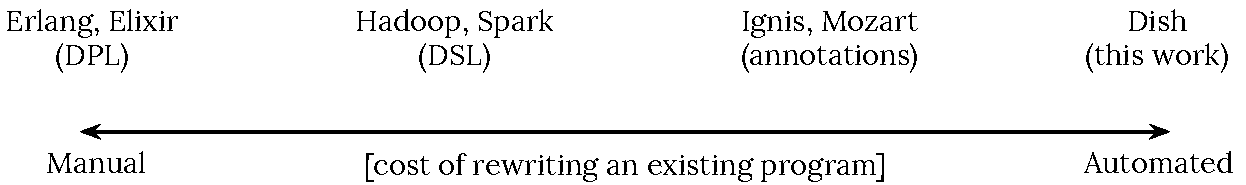
\includegraphics[width=0.49\textwidth]{./figs/dish_spectrum.pdf}
\caption{
  \textbf{Cost of Manual Effort.}
	\sys sits at the automation end of the spectrum, automatically distributing shell pipelines while maintaining their correctness. A more complete picture is presented in the related-work section~\sx{rt}.
}
\label{fig:spectrum}
\end{figure}


\section{Conclusion}
\label{discussion}

\begin{acks}
  % Dumping people so that we don't forget
  % 
  This material is based upon work supported by the
  \grantsponsor{GS100000001}{National Science
    Foundation}{http://dx.doi.org/10.13039/100000001} under Grant
  No.~\grantnum{GS100000001}{nnnnnnn} and Grant
  No.~\grantnum{GS100000001}{mmmmmmm}.  Any opinions, findings, and
  conclusions or recommendations expressed in this material are those
  of the author and do not necessarily reflect the views of the
  National Science Foundation.
\end{acks}


%% Bibliography
\bibliography{./bib}


%% Appendix
\appendix
\section{Scripts used in the evaluation}

This appendix contains the source code of the scripts used in the evaluation of
the \sys. They are part of the codebase (released as open source with the camera
ready), and are provided here only to aid the reviewers.


\end{document}
